%\documentclass[draft]{agujournal2018}
\documentclass[]{agujournal2018}
\usepackage{apacite}
\usepackage{url}
\usepackage{lineno}
%\linenumbers
\draftfalse
\journalname{Geophysical Research Letters}

%custom packages
\usepackage{amsmath,amssymb,amsfonts,amsthm}
\usepackage{comment}
\usepackage{booktabs}
% custom commands
\newcommand\be{\begin{equation}}
\newcommand\ee{\end{equation}} 
\newcommand\bra{\langle}
\newcommand\ket{\rangle}
\newcommand\om{\omega}
\newcommand\tom{\tilde{\omega}}
\newcommand\tg{\tilde{g}}
\newcommand\tp{\tilde{p}}
\newcommand\tG{\tilde{G}}
\newcommand\El{\mathcal{L}}

\begin{document}

\title{Back to Einstein: how to include trapping processes in fluvial diffusion models?}

\authors{James K. Pierce \affil{1}and Marwan A. Hassan\affil{1}}
\affiliation{1}{Department of Geography \\University of British Columbia}
\correspondingauthor{James Kevin Pierce}{kpierce@alumni.ubc.ca}

\begin{keypoints}
\item We generalize the bedload diffusion model of Hans Albert Einstein to include the duration of sediment motion and the possibility of trapping.
\item This derives three stages of bedload diffusion and unambiguously attributes physical mechanisms to each stage.
\end{keypoints}

\begin{abstract}
One approach to predict geomorphic change in rivers is to upscale from the motions of individual sediment grains. A difficulty with this approach is the wide range of individual motion characteristics that imply sediment diffusion, or the spreading out of grains through time. A more acute difficulty is that these motion characteristics apparently vary across temporal and spatial scales, implying multiple stages of sediment diffusion. We relate this multi-stage diffusion to within-channel trapping processes that impede the motions of individual grains. Grains can become stranded on high bars during floods, or they can become buried within the sedimentary bed, but these processes take a relatively long time to occur. Drawing on ideas from condensed matter physics and cellular biology, we describe the finite-velocity motions of individual grains within channels as random walkers subject to trapping. This derives three stages of bedload diffusion and clarifies the underlying mechanism, providing a tool to link between scales.
\end{abstract}

\section{Introduction}


Models to predict the movement patterns of individual bedload sediment grains through rivers have been studied since at least \citet{Einstein1937}.
Einstein originally used a random walk concept to describe these patterns statistically, and he applied his model to experimental data from a series of flume experiments.
Individual movements are ultimately responsible for changes in the spatial organization of river channels \citep{Hassan2017}, so predictive models of these patterns could benefit a vast set of environmental considerations, ranging from aquatic habitat restoration \citep{Hauer2016} to the management of contaminated streams \citep{Macklin2006} and artificial reservoirs \citep{Schleiss2016}.
Unfortunately, Einstein's approach does not provide a definitive solution to this problem, although its essential concepts lie at the base of the majority of contemporary approaches.
The essential issue is that Einstein's original measurements on bedload transport characteristics are now known to be relevant only on a certain observation timescale \citep{Nikora2001a}.
Since \citet{Einstein1937}, details of bedload transport have come to light which are not accessible by his measurement techniques.
There is a need for new models to account for these new details and predict the movements of individual grains.

When bedload grains transport downstream, each grain is imparted a unique sequence of forces by turbulent and steady components of the flow \citep{} and collisions with other moving and stationary grains \citep{Gordon1972}. 
As a result, grains spread apart from one another as they transport downstream: a phenomenon called diffusion.
Diffusion is characterized by the variance of particle position $\sigma_x^2(t)$ \citep{Furbish2017}.
An extreme diversity of transport phenomena show diffusion: it is not limited to the movement of grains within river channels, and it has been deeply studied in geology \citep{Berkowitz2006}, chemistry \citep{Shugard1976}, biology \citep{Sokolov2012}, hydrology \citep{Yang2019}, and many other contexts.
The classic examples are pollen grains diffusing in response to molecular collisions while suspended in water, as first described mathematically by Hans Albert Einstein's father \citep{Einstein1905} and sand within a pipe flow \citep{Taylor1920}.
In these cases, individual particles (pollen, sand, gravel) spread apart at a rate proportional to the time: $\sigma_x^2 \propto t$. Such diffusion is said to be normal.
This name connotes the idea that this diffusion is somehow particularly characteristic of natural phenomena.

In contrast to this nomenclature, researchers of transport phenomena across the physical sciences have realized that normal diffusion is far from ubiquitous \citep{Shlesinger1993}.
When diffusion is not normal, it is called anomalous, a term defined by a variance scaling $\sigma_x^2 \propto t^\gamma$, where $\gamma \neq 1$. 
Some examples of anomalous diffusion include transport of nutrients through lipid bilayers \citep[e.g.][]{Jeon2012,Molina-Garcia2018}, contaminants through groundwater aquifers \citep[e.g.][]{AaraoReis2014,Yang2019}, charge carriers through solids \citep[e.g.][]{Scher1973}, and, indeed, sediment grains through rivers \citep{Hassan2017,Phillips2013,Martin2012,Bradley2017}.
In this work, we revisit the approach of Einstein to bear on the problem of multiple-stage diffusion.
We draw upon methods developed in biology and condensed matter physics to form a description of anomalous and multi-stage diffusion which is directly linked to the original formulation of Einstein.
There is a need to review \citet{Wu2019, Zhang2012, Hassan2017, Phillips2013, Martin2012} and write something meaningful involving them, then rewrite this introduction because it isn't good.
Anyway, here's the model.


\section{Bedload diffusion with trapping}
To include motion, rest, and burial into a model of bedload diffusion, we leverage the mathematical formalism of multi-state random walks.
The multi-state random walk was first considered by \citet{Weiss1976} and is reviewed in \citet{Weiss1994}. Our development closely follows these works and involves two essential stages.
First, we calculate the joint probabilities that a tracer's residence or sojourn within each state ends at time $t$ having position $x$.
Second, we calculate the joint probabilities that a tracer in each state has position $x$ at time $t$ regardless of whether or not a sojourn has just completed.
These two sets of objects completely define the stochastic dynamics of tracers.

Tracers at rest may be trapped by burial.
We consider burial to be permanent \citep[e.g.][]{Wu2019}, and we characterize it probabilistically.
Assuming that resting grains may be buried with constant probability per unit time $\kappa$, the probability that a resting grain is not trapped after a time $t$ is given by a survival probability $\Phi(t) = e^{-\kappa t}$. Likewise, the probability that it is trapped after resting for a time $t$ is the complement $1-\Phi(t)$.
Associating indices $i=0,1,2$ with the trapping, resting, and moving states, we introduce $\omega_{1T}(x,t)$, $\omega_{1F}(x,t)$, and $\omega_2(x,t)$ as the joint probabilities to find a grain having just completed a sojourn at $x,t$.
The subscript ${1T}$ denotes the completion of a rest sojourn due to trapping, while $1F$ denotes the completion of a rest sojourn due to movement.
Similarly, the subscript $2$ denotes the completion of a movement sojourn due to the onset of resting.
We consider that only resting grains can be buried.
Using an argument similar to \citet{Weiss1994}, we can write integral equations to link the $\omega$'s. 
\begin{align}
\om_{1T}(x,t) &= \theta_1\big[1-\Phi(t)\big]g_1(x,t) + \int_0^x dx' \int_0^t dt' \om_2(x',t')\big[1-\Phi(t)\big]g_1(x-x',t-t')\\
\om_{1F}(x,t) &= \theta_1\Phi(t)g_1(x,t) + \int_0^x dx' \int_0^t dt' \om_2(x',t') \Phi(t) g_1(x-x',t-t')\\
\om_2(x,t) &= \theta_2 g_2(x,t) + \int_0^x dx' \int_0^t dt' \om_{1F}(x',t')g_2(x-x',t-t')\\
\end{align}
The factors $g_i(\xi,\tau)$ are called propagators in the state $i$. They encode the transfer of probability across a distance $\xi$ and a time $\tau$ while the walker resides in the $i$th state.
Specifying the propagators and solving these equations for the $\omega$ completes the first stage of the derivation.

The propagators are defined by the behavior of particles in each state.
We consider that sojourns through motion and rest states last for exponentially distributed times.
Since resting particles do not move, while moving particles translate with a constant velocity $v$, we reason the propagators are 
\be g_1(x,t) = \delta(x) k_1e^{-k_1t}\ee
\be g_2(x,t) = \delta(x-vt)k_2e^{-k_2t}.\ee
In this notation, $1/k_1$ is the mean resting time, while $1/k_2$ is the mean movement time.

The second stage of our development involves the joint probabilities of being in state regardless of whether a sojourn has just completed. These are denoted by  $p_0$ (trapped), $p_1$ (rest), and $p_2$ (motion) and involve the $\omega$s for their definition.
\begin{align}
p_0(x,t) &= \int_0^t dt' \omega_{1T}(x,t-t')\\
p_1(x,t) &= \theta_1 G_1(x,t) + \int_0^x dx' \int_0^t dt' \omega_2(x',t')G_1(x-x',t-t')\\
p_2(x,t) &= \theta_2 G_2(x,t) + \int_0^x dx' \int_0^t dt' \omega_{1F}(x',t')G_2(x-x',t-t'),
\end{align},
while the total probability is $p(x,t) = p_0(x,t) + p_1(x,t) + p_2(x,t)$.
When the propagators are chosen as \citet{Lisle1998}, this has solution 
\begin{align}
p(x,t) = &e^{-(\kappa + k_1)(t-x/v)-k_2x/v} \theta(t-x/v)\\
&\times \Bigg[\frac{1}{v}\delta(t-x/v) + \frac{1}{v}\sqrt{\frac{k_1k_2x}{v(t-x/v)}}\mathcal{I}_1\Bigg(2\sqrt{\frac{k_1k_2x}{v}\Big(t-\frac{x}{v}\Big)}\Bigg) +\frac{k_2}{v}\mathcal{I}_0\Bigg(2\sqrt{\frac{k_1k_2x}{v}\Big(t-\frac{x}{v}\Big)}\Bigg) \Bigg]\\
&+ \kappa\frac{ k_2}{v(\kappa+k_1)}\theta(t-x/v)e^{-k_2x/v}\mathcal{P}_1\Big(\frac{k_1k_2x}{v(\kappa+k_1)},[\kappa+k_1][t-x/v] \Big)
\label{eq:pdf}
\end{align}
as shown in appendix \ref{sec:appendix}. The $I_\nu$ are modified Bessel functions of the first kind and $\mathcal{P}_1$ is a Marcum-Q function \citep{Marcum1960,Temme1996}. $\theta(x)$ is the Heaviside step function and we use the convention $\theta(x=0)=1$.
This distribution is depicted in figure \ref{fig:pdfs}.
\begin{figure}
	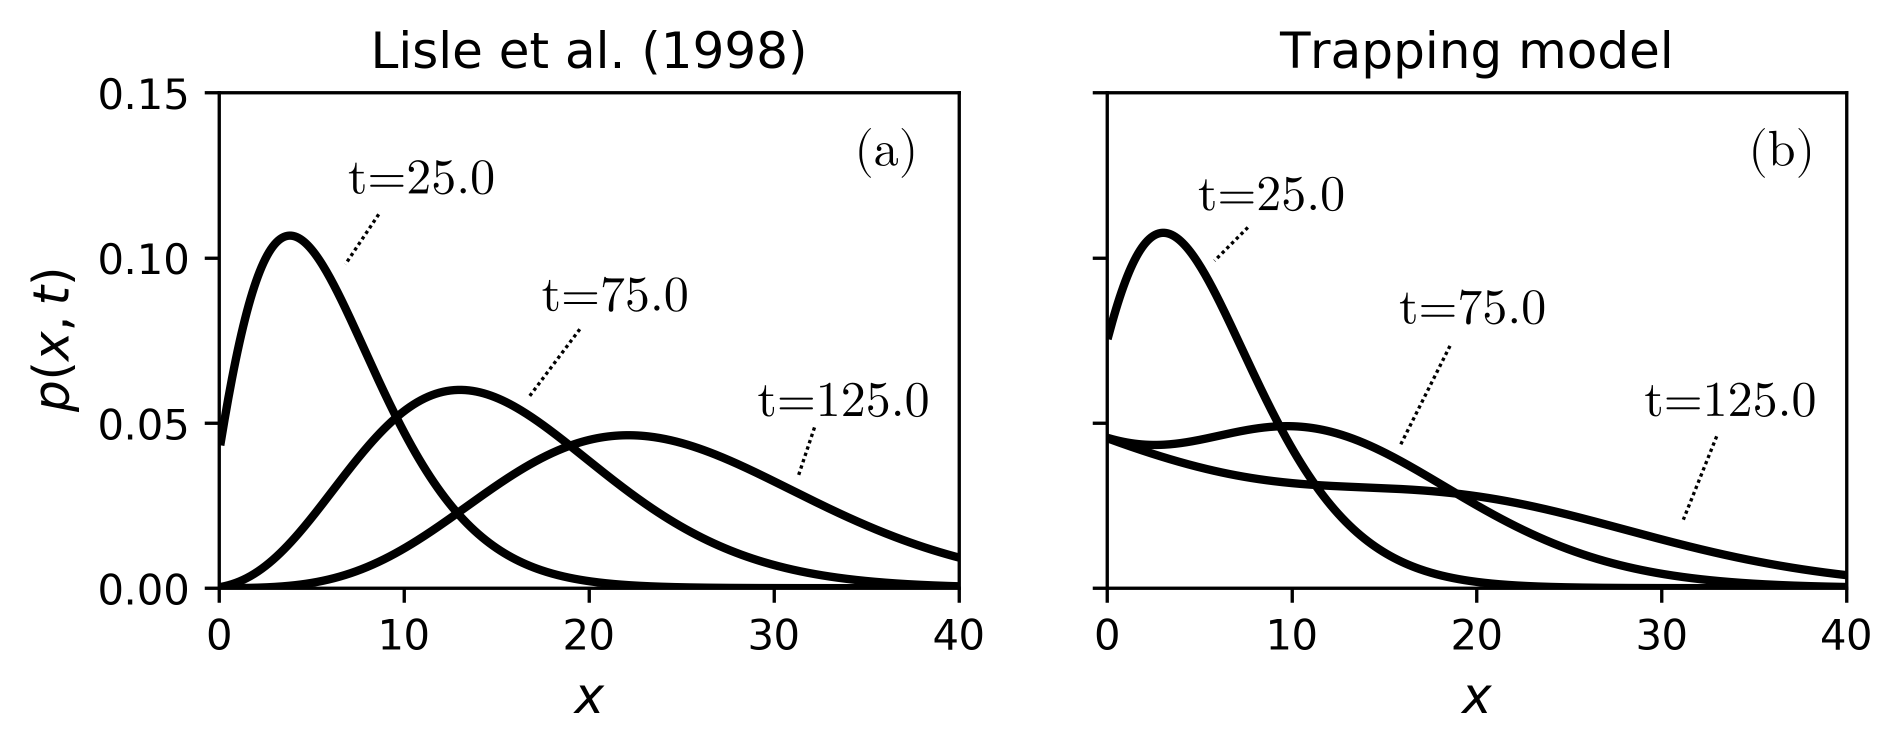
\includegraphics[width=\linewidth,keepaspectratio]{./figures/pdf-plot-edit.png}
	\caption{Joint distributions of a tracer being found at $x$ $t$ are impeded by the trapping process. Panel (a) shows the \citet{Lisle1998} model, and panel (b) shows the the distribution \ref{eq:pdf} which results from a trapping process occurring at rate $\kappa$. Cross-comparison of both panels shows that trapping redistributes probability to smaller values of $x$, and this redistribution becomes more important for larger $t$.}
	\label{fig:pdfs}
\end{figure}
The key tool in the analysis in the appendices is the double-Laplace transform of functions which depend on space and time:
\be \hat{f}(\eta,s) = \int_0^\infty dx \int_0^\infty ds e^{-st-\eta x}f(x,t).\ee
This unravels the convolution structure in the equations and provides an alternative approach to calculate the moments of $x$ which avoids integrating (\ref{eq:pdf}).
This approach is based on taking derivatives of $\hat{p}(\eta,s)$ as described in appendix \ref{sec:appendix2}.
The first two moments are
\be \bra x(t) \ket = A_1 e^{(b-a)t}+B_1e^{-(a+b)t}+C_1 \label{eq:mean}\ee
\be \bra x^2(t) \ket = A_2(t)e^{(b-a)t}+B_2(t)e^{-(a+b)t}+C_2, \label{eq:second}\ee
where $A_i$ and $B_i$ are polynomials tabulated in (\ref{table:params}).
The operator $\bra \circ \ket$ denotes the ensemble average \citep[e.g.][]{Kittel1958}.
In terms of these moments, the variance $\sigma_x^2 = \bra x^2\ket - \bra x \ket^2$ is
\be \sigma_x^2(t) = A(t)e^{(b-a)t} + B(t)e^{-(a+b)t} + C(t) \label{eq:var}\ee
We have made no approximation to derive this expression, so it represents the phenomena of a \citet{Lisle1998}-type model generalized to include sediment trapping processes.
\begin{table}[!h]
\centering
\caption{Polynomials and transcendental functions used in the expressions of the mean (\ref{eq:mean}), second moment (\ref{eq:second}) and variance (\ref{eq:var}) of bedload tracers.}
\label{table:params}
\begin{tabular}{c}
\toprule
$A_1 = \frac{v}{2b}\big[1+\frac{\kappa+k_1}{b-a}\big]$ \\
$B_1 = -\frac{v}{2b}\big[1-\frac{\kappa+k_1}{a+b}\big]$ \\
$C_1 =  -\frac{v}{2b}\big[\frac{\kappa+k1}{b-a}+\frac{\kappa+k1}{a+b}\big]$\\
$A_2(t)=\frac{v^2}{2b^3}\Big[b+(b-a)[bt-1]+2(\kappa+k_1)[bt-1] + \frac{(\kappa+k_1)^2}{(a-b)^2}[-abt+a+b(bt-2)]\Big] $\\
$B_2(t) = \frac{v^2}{2b^3}\Big[b-(a+b)[bt+1]+2(\kappa+k_1)[bt+1] - \frac{(\kappa+k_1)^2}{(a+b)^2}[bt(a+b)+a+2b]\Big] $\\
$C_2(t) = \frac{v^2}{2b^3}(\kappa+k_1)^2\Big[\frac{a+2b}{(a+b)^2}+\frac{-a+2b}{(a-b)^2}\Big]$\\
$A(t) = A_2(t)-2A_1C_1 + A_1^2\exp[(b-a)t]$\\
$B(t) = B_2(t)-2B_1C_1 + B_1^2\exp[-(a+b)t]$\\
$C(t) = C_2-C_1^2+2A_1B_1\exp[-2at]$\\
\bottomrule
\end{tabular}
\end{table}


\section{Discussion: new findings and foundational links}
A plot of $\sigma_x^2(t)$ is shown in figure \ref{fig:var}.
\begin{figure}
	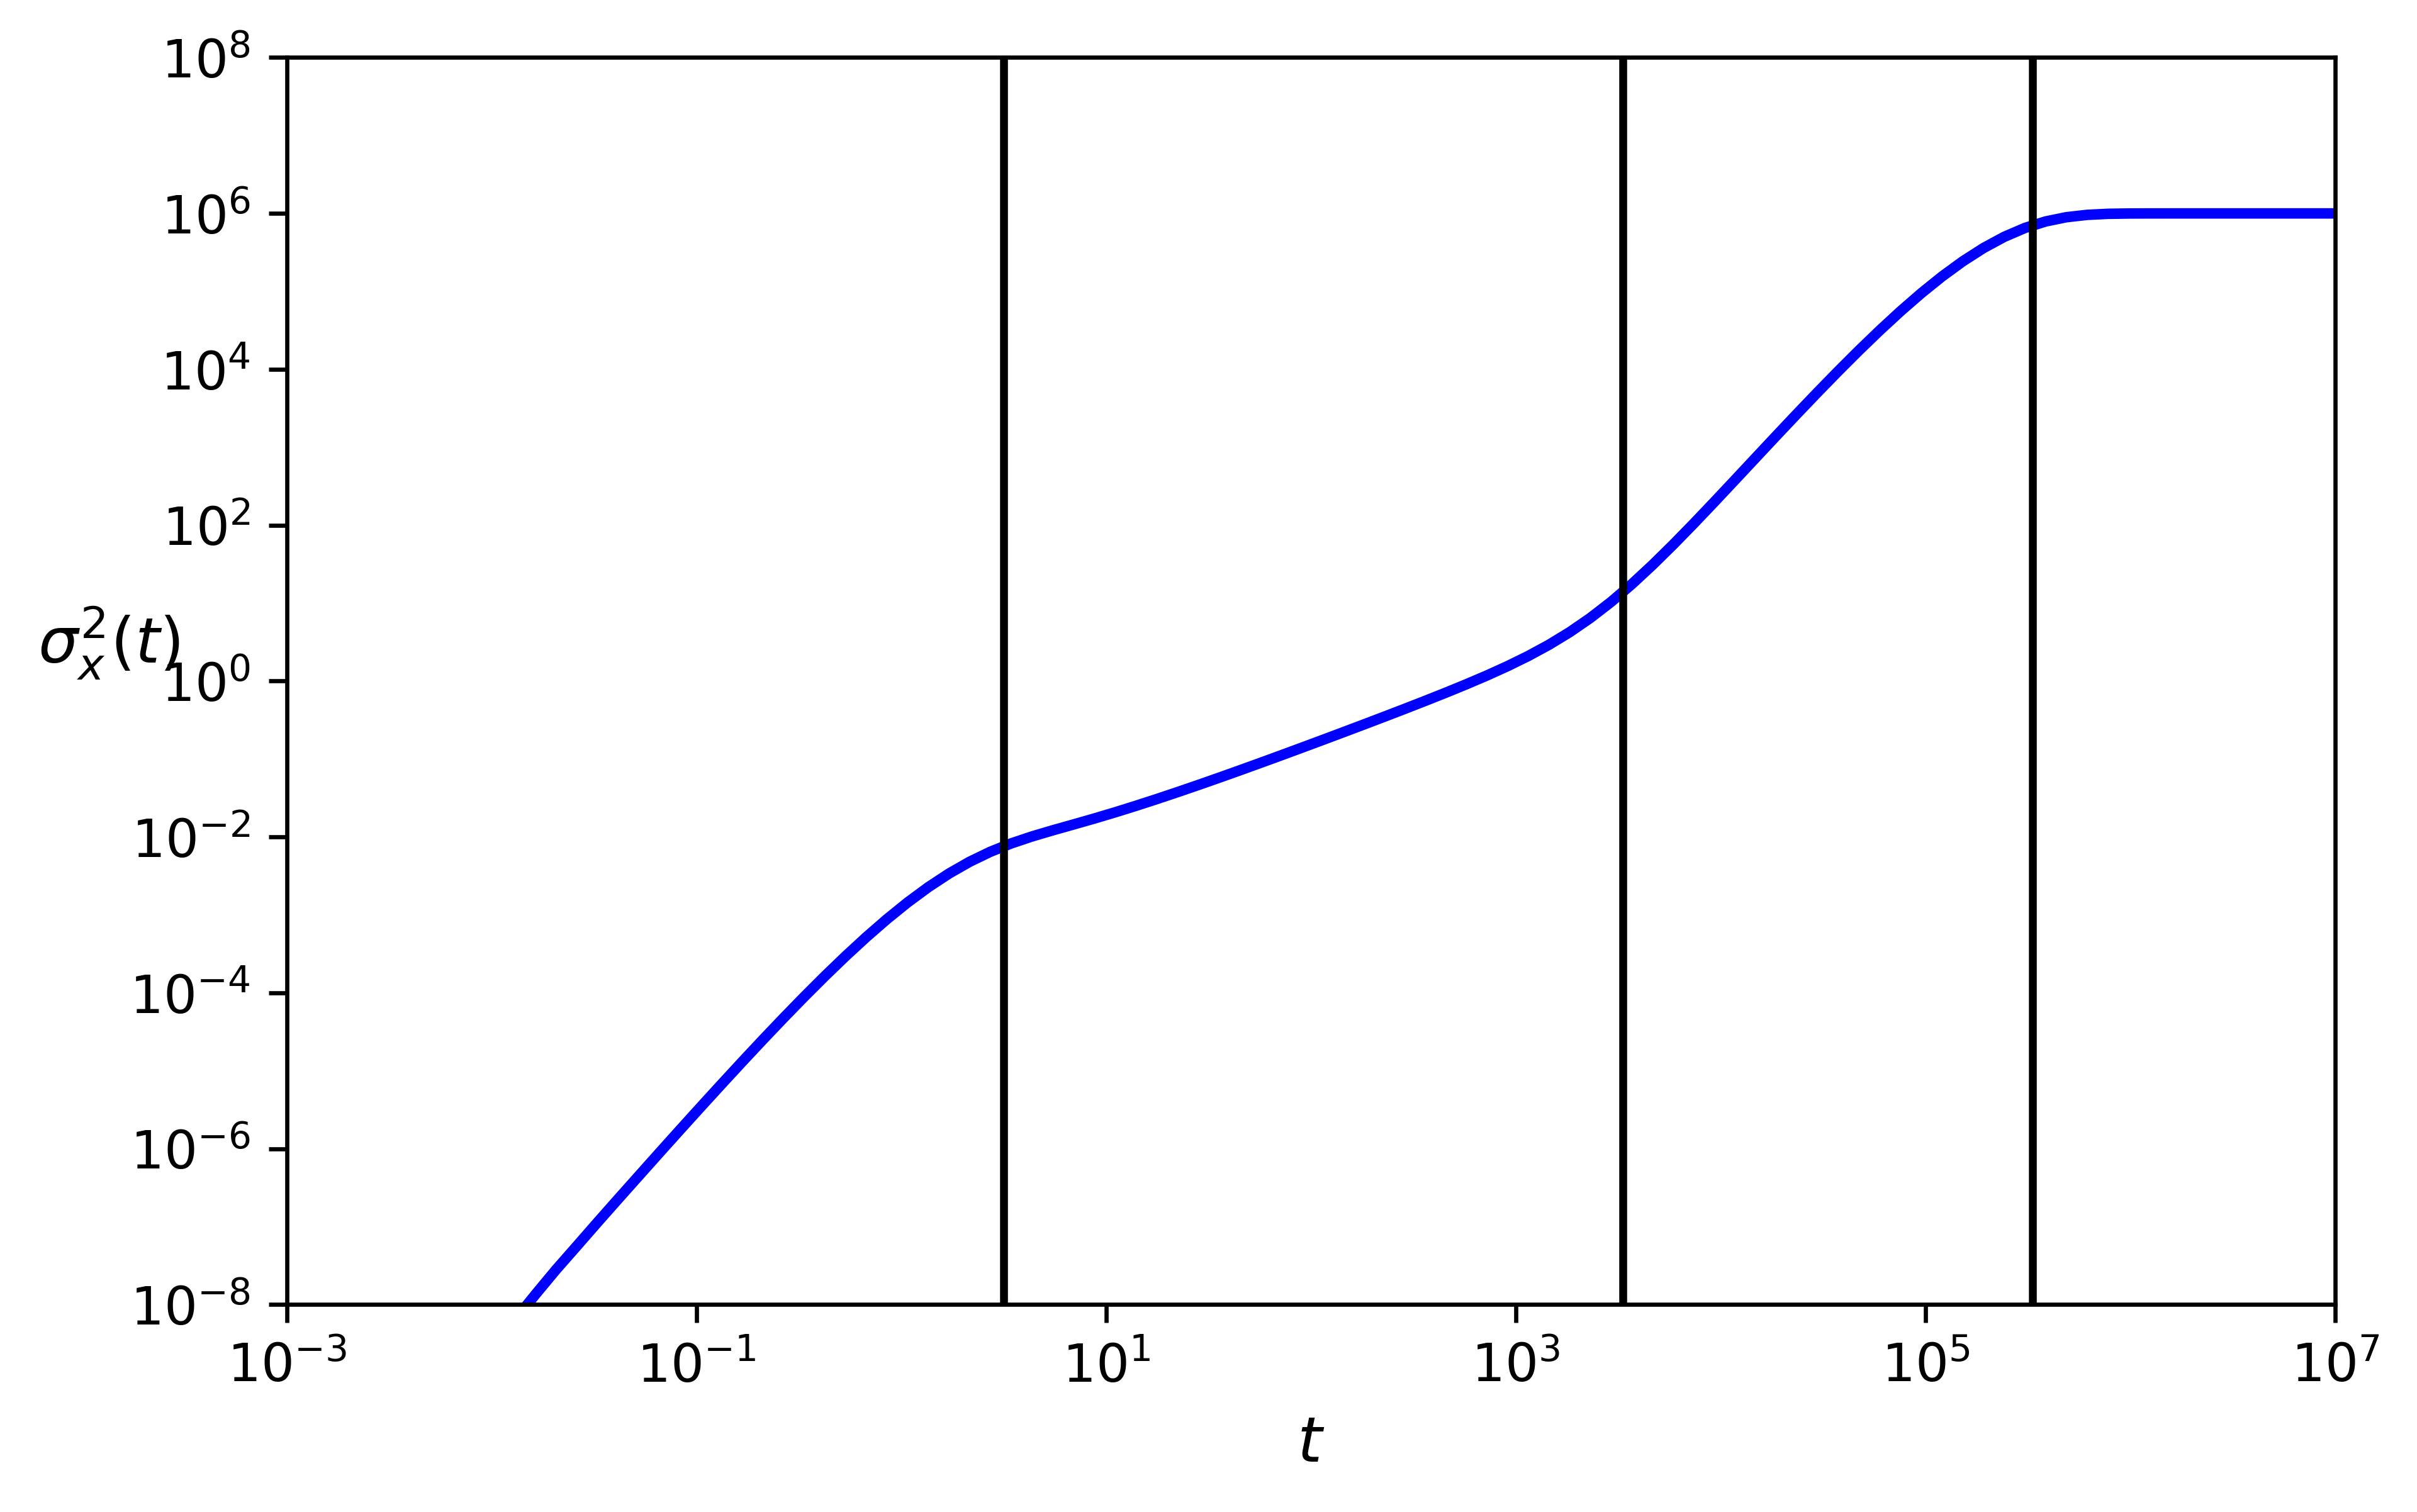
\includegraphics[width=\linewidth,keepaspectratio]{./figures/diffusion.png}
	\caption{The variance of tracer position exhibits four distinct scaling regions as time increases: local, intermediate, global, and finally a non-diffusive range characterized by the eventual trapping of all grains.
	Local and global ranges show super-diffusion $\sigma_x^2 \propto t^3$ while the intermediate range shows normal diffusion. These conclusions hold only for $\kappa \ll k_1 \ll k_2$, meaning motion intervals are generally much shorter than resting intervals, which are in turn are generally much smaller than the time required for resting particles to become buried.}
	\label{fig:var}
\end{figure}


\section{Conclusion}


\appendix

\section{Calculation of the distribution function with trapping}
\label{sec:appendix}
Taking double transforms gives
\begin{align}
\tom_{1T}(\eta,s) &= \theta_1 \tg_1(\eta,s) + \tom_2(\eta,s)\tg_1(\eta,s)-\tom_{1F}(\eta,s) \\
\tom_{1F}(\eta,s) &= \theta_1\tg_1(\eta,s+\kappa) + \tom_2(\eta,s)\tg_1(\eta,s+\kappa)\\
\tom_2(\eta,s) &= \theta_2 \tg_2(\eta,s) + \tom_{1F}(\eta,s)\tg_2(\eta,s)
\end{align}
This system solves for 
\begin{align}
\tom_{1T}(\eta,s) &= \frac{\theta_1 + \theta_2 \tg_2(\eta,s)}{1-\tg_1(\eta,s+\kappa)\tg_2(\eta,s)}\big\{\tg_1(\eta,s)-\tg_1(\eta,s+\kappa) \big\} \\
\tom_{1F}(\eta,s) &= \frac{\theta_1 + \theta_2 \tg_2(\eta,s)}{1-\tg_1(\eta,s+\kappa)\tg_2(\eta,s)}\tg_1(\eta,s+\kappa)\\
\tom_{2}(\eta,s) &= \frac{\theta_2 + \theta_1 \tg_1(\eta,s+\kappa)}{1-\tg_1(\eta,s+\kappa)\tg_2(\eta,s)}\tg_2(\eta,s)\\
\end{align}


The probabilities of being in state $0$ (trapped), $1$ (rest), and $2$ (motion) are
\begin{align}
p_0(x,t) &= \int_0^t dt' \omega_{1T}(x,t-t')\\
p_1(x,t) &= \theta_1 G_1(x,t) + \int_0^x dx' \int_0^t dt' \omega_2(x',t')G_1(x-x',t-t')\\
p_2(x,t) &= \theta_2 G_2(x,t) + \int_0^x dx' \int_0^t dt' \omega_{1F}(x',t')G_2(x-x',t-t'),
\end{align}
Double transforming gives
\begin{align}
\tp_0(\eta,s) &= \frac{1}{s}\tom_{1T}(\eta,s)\\
\tp_1(\eta,s) &= \theta_1 \tG_1(\eta,s) + \tom_2(\eta,s) \tG_1(\eta,s) \\
\tp_2(\eta,s) &= \theta_2 \tG_2(\eta,s) + \tom_{1F}(\eta,s)\tG_2(\eta,s)\\
\end{align}
The total probability is $p(x,t) = p_0(x,t) + p_1(x,t) + p_2(x,t)$ or 
\begin{multline}
\tp(\eta,s) = \frac{1}{s}\frac{\theta_1 + \theta_2 \tg_2(\eta,s)}{1-\tg_1(\eta,s+\kappa)\tg_2(\eta,s)}\big\{\tg_1(\eta,s)-\tg_1(\eta,s+\kappa) \big\} \\
+\frac{\theta_1\big[\tG_1(\eta,s) + \tg_1(\eta,s+\kappa)\tG_2(\eta,s)\big]+ \theta_2\big[\tG_2(\eta,s) + \tg_2(\eta,s)\tG_1(\eta,s)\big]}{1-\tg_1(\eta,s+\kappa)\tg_2(\eta,s)} \\
\end{multline}
Using the identities $\tg_i(0,s) = \tilde{\psi}_i(s)$ and $\tG_i(0,s) = (1-\tilde{\psi}_i(s))/s,$ it follows that the joint distribution is normalized in space: $\tp(0,s) = \mathcal{L}\{\int_0^\infty dx p(x,t);s\} = 1/s$.

After a lot of work which is in your notebook, this becomes
\begin{align}
p(x,t) = e^{-(\kappa + k_1)(t-x/v)-k_2x/v}
\Big[&\frac{1}{v}\El_{s\rightarrow t-x/v}^{-1}\Big\{\exp\Big[\frac{k_1k_2}{vs}x\Big]\Big\} \\
&+ \frac{k_2}{v}\El_{s\rightarrow t-x/v}^{-1}\Big\{\frac{1}{s}\exp\Big[\frac{k_1k_2}{vs}x\Big]\Big\} \\
&+ \frac{\kappa k_2}{v}\El_{s\rightarrow t-x/v}^{-1}\Big\{\frac{1}{(s-\kappa-k_1)s}\exp\Big[\frac{k_1k_2}{vs}x\Big]\Big\}\Big]
\end{align}
\begin{align}
p(x,t) = e^{-(\kappa + k_1)(t-x/v)-k_2x/v}
\Bigg[&\frac{1}{v}\delta(t-x/v) + \frac{1}{v}\sqrt{\frac{k_1k_2x}{v(t-x/v)}}\theta(t-x/v)\mathcal{I}_1\Bigg(2\sqrt{\frac{k_1k_2x}{v}\Big(t-\frac{x}{v}\Big)}\Bigg)\\
&+\frac{k_2}{v}\theta(t-x/v)\mathcal{I}_0\Bigg(2\sqrt{\frac{k_1k_2x}{v}\Big(t-\frac{x}{v}\Big)}\Bigg)\\
&+ \kappa\frac{ k_2}{v(\kappa+k_1)}e^{(\kappa+k_1)(t-x/v)}\theta(t-x/v)\mathcal{F}(x,t)\Bigg]
\end{align}
where the function $\mathcal{F}$ is
\be \mathcal{F}(x,t) = \sum_{j=0}^\infty \frac{\big[\frac{k_1k_2x}{v(\kappa+k_1)}\big]^j}{j!j!} \gamma\big(j+1,[\kappa+k_1][t-x/v]\big),\ee
where the $\mathcal{I}_\nu(z)$ are modified Bessel functions of the first kind, and $\gamma(\alpha,z)$ is the lower incomplete gamma function.
This function $\mathcal{F}(x,t)$ is the Marcum Q-function \citep{Temme1996}, given by 
\be \mathcal{Q}_1(x,y) = 1-e^{-x}\sum_{n=0}^\infty \frac{x^n}{n!}\frac{\gamma(1+n,y)}{\Gamma(n+1)}\ee
This function was originally introduced in relation to radar detection problems \citep[e.g.][]{Marcum1960}. It has a representation as an infinite superposition of modified Bessel functions:
\be \mathcal{Q}_1(x,y) = 1- \int_0^ydz e^{-z-x}\mathcal{I}_0(2\sqrt{xz})\ee
So we are not far from where we started with \citet{Lisle1998}: Modified Bessel functions are the norm in this type of 1D diffusion problem \citep[e.g.][]{Lisle1998}.
Hence in summary \be \mathcal{F}(x,t) = 1-\mathcal{Q}_1\Big(\frac{k_1k_2x}{v(\kappa+k_1)},[\kappa+k_1][t-x/v] \Big)\ee

\section{Calculation of the moments}
\label{sec:appendix2}
Often, Tauberian-type theorems are used to study the long or short time asymptotic scaling of first or second moments of random walks having any generality.
This is because the mathematics get difficult, and Tauberian theorems provide a very powerful tool which leverages the stability of the Laplace transform.
Unfortunately, this approach is insufficient for our purposes. We are unaware of an intermediate-regime Tauberian-type theorem, so we must pursue full solutions of the moments in order to discriminate the diffusive ranges and the full diffusion behavior.

\be \partial_\eta \tp(\eta,s) = -v \frac{1}{s}\frac{[(s+\kappa + k')s + \kappa k_2][s+\kappa + k_1]}{[\eta v(s+\kappa +k_1) + (s+ \kappa + k')s+\kappa k_2]^2}\ee
\be \partial_\eta^2 \tp(\eta,s) = 2v^2 \frac{1}{s} \frac{[(s+\kappa + k')s+\kappa k_2][s+\kappa + k_1]^2}{[\eta v(s+\kappa + k_1) + (s+\kappa + k')s+ \kappa k_2]^3}\ee
\be  \frac{\bra\tilde{x}\ket} {v} = \frac{1}{s}\frac{s+\kappa + k_1}{(s+\kappa + k')s + \kappa k_2}\ee
\be \frac{\bra \tilde{x}^2 \ket}{2v^2} = \frac{1}{s} \frac{[s+\kappa + k_1]^2}{[(s+\kappa + k')s + \kappa k_2]^2} \ee

A similar approach provides 
\begin{align}
\frac{\bra x^2 \ket}{2v^2} &= \Big(\frac{d}{dt}\circ + \circ \Big|_{t=0} + 2(\kappa + k_1)\circ + (\kappa+k_1)^2\int_0^t dt \circ \Big)\El^{-1}\Big\{\frac{1}{[(s+a)^2-b^2]^2};t\Big\}\\
&= \Big(\frac{d}{dt}\circ + \circ \Big|_{t=0} + 2(\kappa + k_1)\circ + (\kappa+k_1)^2\int_0^t dt \circ \Big)\El^{-1}\Big\{\frac{1}{[s^2-b^2]^2};t\Big\}e^{-at}\\
&= \Big(\frac{d}{dt}\circ + \circ \Big|_{t=0} + 2(\kappa + k_1)\circ + (\kappa+k_1)^2\int_0^t dt \circ \Big)e^{-at}\frac{1}{2b^3}\Big[bt\cosh(bt)-\sinh(bt)\Big]
\end{align}
using Prudnikov 2.1.5.6.
This becomes
\begin{align}
\frac{\bra x^2 \ket}{2v^2} = \frac{t}{b}\sinh&(bt) + \frac{(\kappa + k_1)}{b^3}\big[bt\cosh(bt)-\sinh(bt)\big]\\
&+e^{-at}\frac{b(b^2(at-2))-a^3t)\cosh(bt) +(a^3-a^2b^2t-3ab^2+b^4t)\sinh(bt)}{(a-b)^2(a+b)^2}
\end{align}
\begin{align}
\frac{\bra x \ket}{v} &= \El^{-1}\Big\{\frac{1}{s}\frac{s+\kappa + k_1}{(s+\kappa + k')s + \kappa k_2};t\Big\} \\
&= \El^{-1}\Big\{\frac{1}{\big[s+\frac{\kappa+k'}{2}\big]^2+\kappa k_2 - \big[\frac{\kappa+k'}{2}\big]^2};t\Big\} + 
\int_0^t du \El^{-1}\Big\{\frac{\kappa + k_1}{\big[s+\frac{\kappa+k'}{2}\big]^2+\kappa k_2 - \big[\frac{\kappa+k'}{2}\big]^2};u\Big\}\\
&= e^{-(\kappa + k')t/2}\El^{-1}\Big\{\frac{1}{s^2 - b^2};t\Big\} + (\kappa + k_1)\int_0^t du e^{-(\kappa + k')u/2}\El^{-1}\Big\{\frac{1}{s^2 - b^2};u\Big\}
\end{align}
here $b^2 = -\kappa k_2 + \big[\frac{\kappa+k'}{2}\big]^2$
Then with Prudnikov 2.1.5.4:
\begin{align}
\frac{\bra x \ket}{v} &= \frac{1}{b}e^{-(\kappa + k')t/2}\sinh(bt) + \frac{(\kappa +k_1)}{b}\int_0^t due^{-(\kappa + k')u/2}\sinh(bu)\\
&=  \frac{1}{b}e^{-at}\sinh(bt) + \frac{\kappa + k_1}{2b}\Big[\frac{1}{b-a}\Big(e^{(b-a)t}-1\Big)+ \frac{1}{a+b}\Big(e^{-(a+b)t}-1\Big)\Big]
\end{align}
where $a=(\kappa + k')/2$ and $b = \sqrt{a^2 -\kappa k_2}$. We are interested in the domain that $a\geq \sqrt{\kappa k_2}$ so that $b\geq a$.
The limit of $\kappa \rightarrow 0$ provides
\be \frac{k'^2}{v}\bra x \ket=k_2(1-e^{-k't})+ k_1k't \ee
which aligns perfectly with earlier results.

\section{Links to \citet{Einstein1937} and \citet{Lisle1998}}
\acknowledgments
J. Pierce acknowledges helpful exchanges with Eduardo Daly and Peter Hanggi during the early stages of this work. M. Hassan is supported by an NSERC Discovery grant. All simulation code is available on request.

\bibliography{biblio.bib}
\end{document}